\documentclass[UTF-8, a4paper, 12pt]{ctexart}
\usepackage[left=1in,right=1in,top=1.00in,bottom=1.00in]{geometry}% 页边距
\usepackage[colorlinks,linkcolor=blue,anchorcolor=blue,citecolor=green,CJKbookmarks=True]{hyperref}
\usepackage{CJK,CJKnumb}
\usepackage{indentfirst}        % 首行缩进宏包
\usepackage{latexsym,bm}        % 处理数学公式中和黑斜体的宏包
\usepackage{amsmath,amssymb}     % AMSLaTeX宏包 用来排出更加漂亮的公式
\usepackage{graphicx}
\usepackage{cases}
\usepackage{pifont}
\usepackage{txfonts}
\usepackage{subfigure}
\usepackage{pdfpages}
\usepackage{listings}
\usepackage{xcolor}
\usepackage[subfigure]{tocloft}     % 模板中用了subfigure,不加此选项会产生冲突
\usepackage{inconsolata}
\CTEXsetup[format={\Large\bfseries}]{section}%设置章标题字号为Large,居左
\zihao{-4}\linespread{1.5}\selectfont
\renewcommand{\theequation}{\arabic{section}-\arabic{equation}}
\renewcommand{\thefigure}{\arabic{section}-\arabic{figure}}
%\renewcommand{\thefigure}{\thechapter-\arabic{figure}}
\renewcommand{\cftsecleader}{\cftdotfill{\cftdotsep}}
\renewcommand\contentsname{{\qquad\qquad\qquad\qquad\qquad\qquad 目\quad 录}}
\newcommand{\song}{\CJKfamily{song}}    % 宋体   (Windows自带simsun.ttf)
\renewcommand{\abstractname}{\textbf{\large {摘\quad 要}}} %更改摘要二字的样式

%%%%%%%%%%%%%%%%%%%%%%%
% -- text font --
% compile using Xelatex
%%%%%%%%%%%%%%%%%%%%%%%
% -- 中文字体 --
%\setCJKmainfont{Microsoft YaHei}  % 微软雅黑
%\setCJKmainfont{YouYuan}  % 幼圆
%\setCJKmainfont{NSimSun}  % 新宋体
%\setCJKmainfont{KaiTi}    % 楷体
\setCJKmainfont{SimSun}   % 宋体
%\setCJKmainfont{FangSong}   % 仿宋
%\setCJKmainfont{SimHei}   % 黑体
 
% -- 英文字体 --
%\setmainfont{Times New Roman}
%\setmainfont{DejaVu Sans}
%\setmainfont{Latin Modern Mono}
%\setmainfont{Consolas}


%%%%%%%%%%%%%%%%%%%%%%%
%  设置水印
%%%%%%%%%%%%%%%%%%%%%%%
%\usepackage{draftwatermark}         % 所有页加水印
%\usepackage[firstpage]{draftwatermark} % 只有第一页加水印
%\SetWatermarkText{Copyright(C) 2021. by HU S K}           % 设置水印内容
% \SetWatermarkText{\includegraphics{fig/ZJDX-WaterMark.eps}}         % 设置水印logo
%\SetWatermarkLightness{00.9}             % 设置水印透明度 0-1
%\SetWatermarkScale{0.4}                   % 设置水印大小 0-1
%%%%%%%%%%%%%%%%%%%%%%%




%%%%%%%%%%%%%%%%%%%%%%%%%%%%%%%%%%%%%%%%%%%
%用来设置附录中代码的样式
% 头文件
%%%%%%%%%%%%%%%%%%%%%%%%%%%%%%%%%%%%%%%%%%%
\usepackage{listings}
\usepackage{fontspec}
\setmonofont{Consolas}
%\begin{lstlisting}[
%	language = matlab, numbers=left, 
%	numberstyle=\tiny,keywordstyle=\color{blue!70},
%	commentstyle=\color{red!50!green!50!blue!50},frame=shadowbox,
%	rulesepcolor=\color{red!20!green!20!blue!20},
%	basicstyle=\ttfamily,
%	]
%	
%\end{lstlisting}



\title{\bfseries \Huge 基于Python实现NMEA-0183协议下GPS数据的串口通讯程序设计及可视化}
\author{胡森康1120183150}
\date{}

\begin{document}
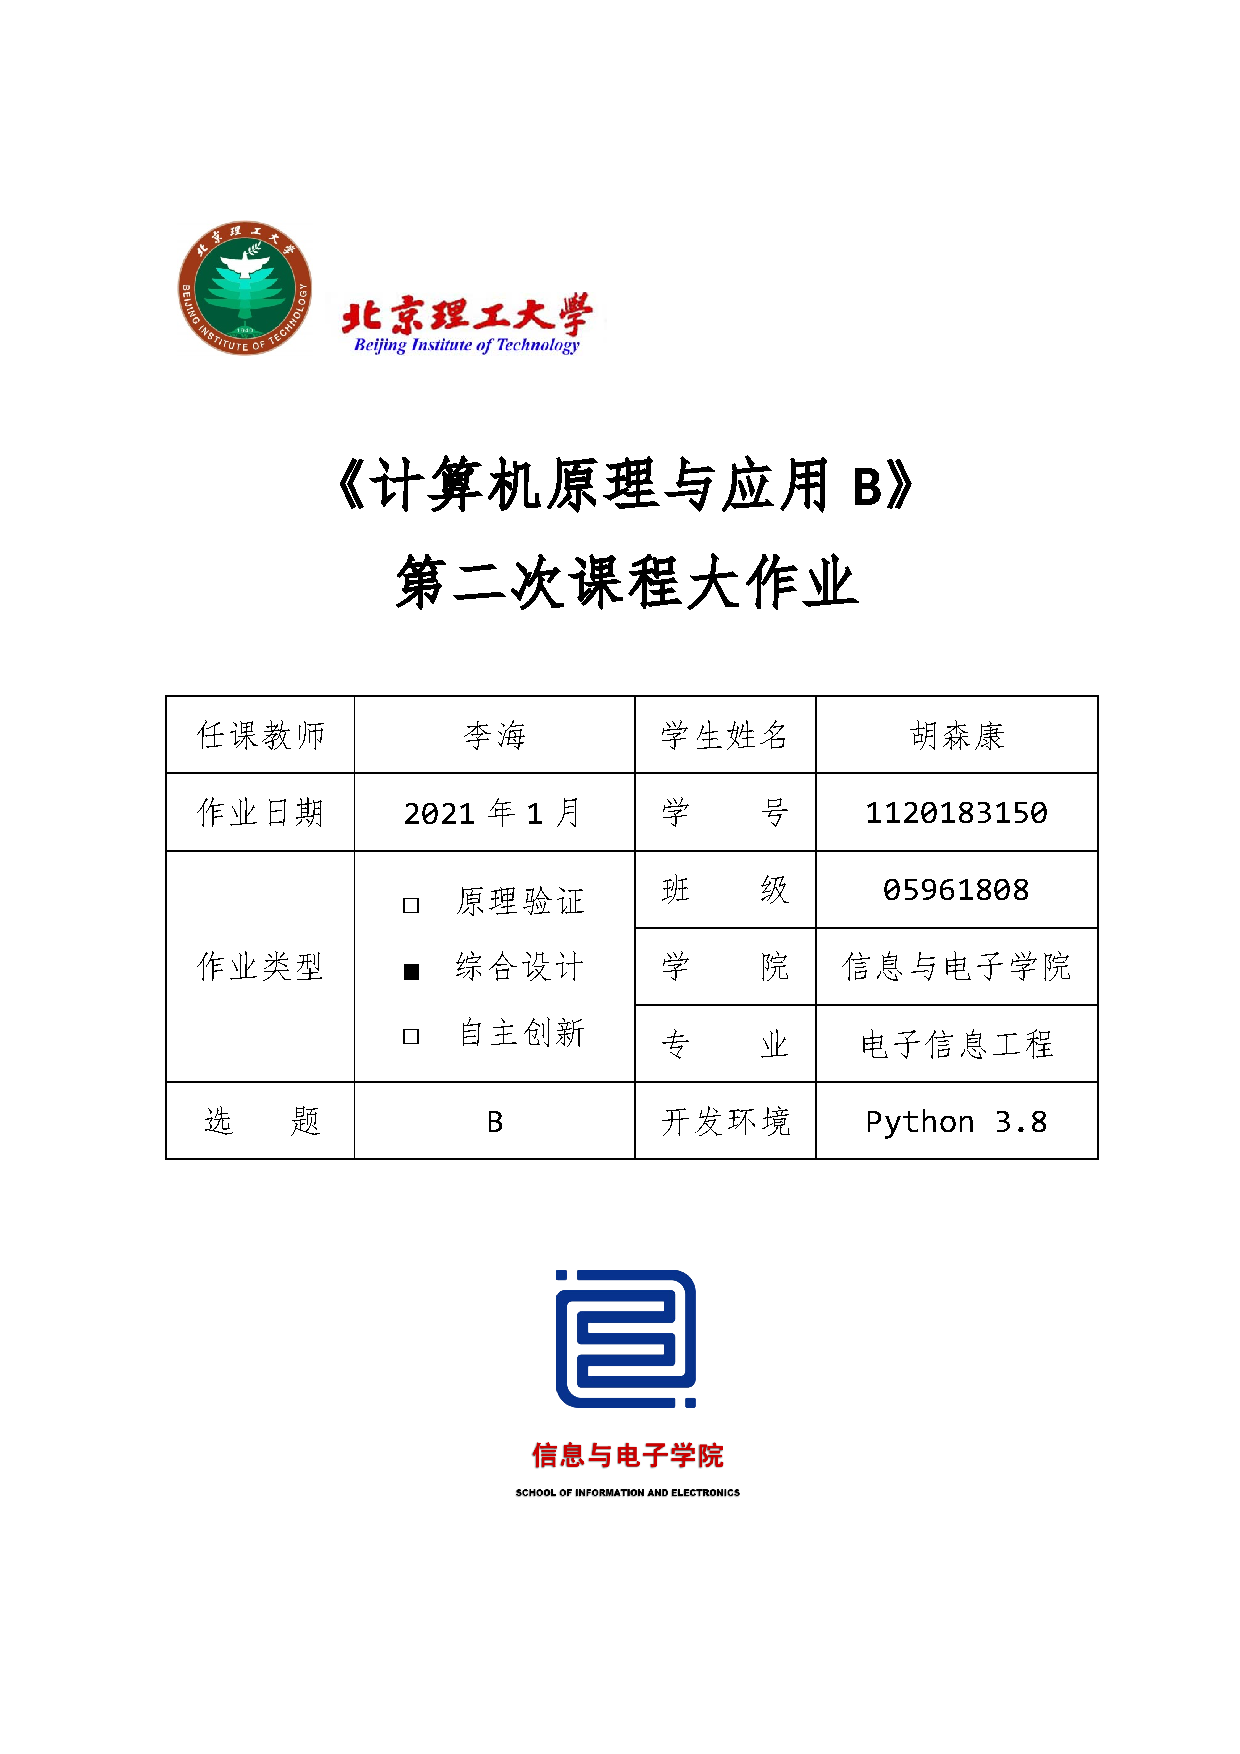
\includepdf[pages={1}]{coverpage.pdf} %% 插入pdf

\maketitle

%\thispagestyle{empty}
%\newpage
%\thispagestyle{empty}
\bigskip
\bigskip
\begin{center}
    {\large 摘\qquad 要}
\end{center}

本项目搭建了虚拟串口环境,同时利用GPS模拟器产生虚拟GPS数据。
并利用Python从虚拟串口读入此数据,
提取虚拟GPS数据中的经纬度,并进行可视化显示。

本文详细阐述了搭建虚拟串口环境的流程,以及调试串口的方法;另外详细
介绍了NEMA-0183协议,以及利用Python从串口导入GPS模拟器
产生的基于NEMA-0183协议的GPS数据的思路和程序;
\bigskip

关键词:GPS\quad Python\quad 串口\quad 可视化\quad NEMA-0183协议
     

     
\thispagestyle{empty}       %本页不显示页码
\newpage                    %分页
\tableofcontents\thispagestyle{empty}
\newpage
\setcounter{page}{1}        %从下面开始编页,页脚格式为导言部分设置的格式



\section{项目背景}
倾覆沉没的钻井平台,顺流直冲的运油车头,直坠入海的满载客机。交通海
上应急反应特勤队第一时间抵达,站在水火咆哮的最前面,守在危急撤离的最后
面,用生命对抗天灾人祸。但在自然面前,特勤员毕竟没有超能力,血肉之躯踩
在死亡边缘,真实的恐惧无数次让这些斗士颤抖、无助和气馁。而海上救援的字
典里没有“退缩”。特勤队有一个GPS 接收机报告当前的位置,但是GPS 接收机
的屏幕被打坏了,只能从GPS 接收机的串口读取位置数据。

GPS 接收机有一个
RS232 串口用来输出数据,接口参数为:波特率为9600,8 位数据位,1 位停止
位,没有校验位。

在此背景下,本项目致力于开发出一款APP,可以从GPS接收机串口读入数据,
并进行可视化显示,以解决特勤队的困难处境。

\section{基本理论}

\subsection{NEMA-0183协议简介}
NMEA-0183是美国国家海洋电子协会(National Marine Electronics Association)
为统一海洋导航规范而制定的标准,该格式标准已经成为国际通用的一种格式,
协议的内容在兼容NMEA-0180和NMEA-0182的基础上,增加了GPS、测深仪、
罗经方位系统等多种设备接口和通讯协议定义,同时还允许一些特定厂商对
其设备通信自定协议(如Garmin GPS,Deso 20等)。NMEA-0183格式数据
串的所有数据都采用ASCII文本字符表示,数据传输以“\$”开头,后面是语句头。
语句头由五个字母组成,分为两部分,前两个字母表示“系统ID”,即表示该语句是属
于何种系统或设备,后三个字母表示“语句ID”,表示该语句是关于何方面的数据。
语句头后是数据体,包含不同的数据体字段,语句末尾为校验码(可选),以回车换
行符<CR><LF>结束,也就是ASCII字符“回车”(十六进制的0DH)和“换行”(十六进制的0AH)。
每行语句最多包含82个字符(包括回车换行符和\$”符号)。数据字段以逗号
分隔识别,空字段保留逗号。以GPS的GPRMC语句为:\bigskip
$$
\begin{array}{l}
    \$GPRMC,<1>,<2>,<3>,<4>,<5>,<6>,<7>,\\ <8>,<9>,<10>,<11>,<12>*hh<CR><LF>
\end{array}
$$

\bigskip
其中GP表示该语句是GPS定位系统的,RMC表示该语句输出的是GPS定位信息,后面是
数据体。最后校验码*hh是用做校验的数据。在通常使用时,它并不是必须的,但
是当周围环境中有较强的电磁干扰时,则推荐使用。hh代表了“\$”和“*”的所有
字符的按位异或值(不包括这两个字符)。个别厂商自己定义语句格式以“\$P”开头
,其后是3个字符的厂家ID识别号,后接自定义的数据体。

\subsection{NEMA-0183协议举例说明}
以下面的GPRMC语句为例:
$$
\$GPRMC,024813.640,A,3158.4608,N,11848.3737,E,10.05,324.27,150706,,,A*50
$$

字段0:\$GPRMC,语句ID,表明该语句为Recommended Minimum Specific GPS/TRANSIT Data(RMC)推荐最小定位信息

字段1:UTC时间,hhmmss.ss格式

字段2:状态,A=定位,V=未定位

字段3:纬度dddmm.mmmm,度分格式(前导位数不足则补0)

字段4:纬度N(北纬)或S(南纬)

字段5:经度dddmm.mmmm,度分格式(前导位数不足则补0)

字段6:经度E(东经)或W(西经)


字段7:速度,节,Knots

字段8:方位角,度

字段9:UTC日期,DDMMYY格式

字段10:磁偏角,(000 - 180)度(前导位数不足则补0)

字段11:磁偏角方向,E=东,W=西

字段16:校验值$\text{}^{[1]}$

\section{搭建虚拟环境}
搭建虚拟环境的流程图如图(\ref{f1})所示。
\begin{figure}[htbp]
    \centering
    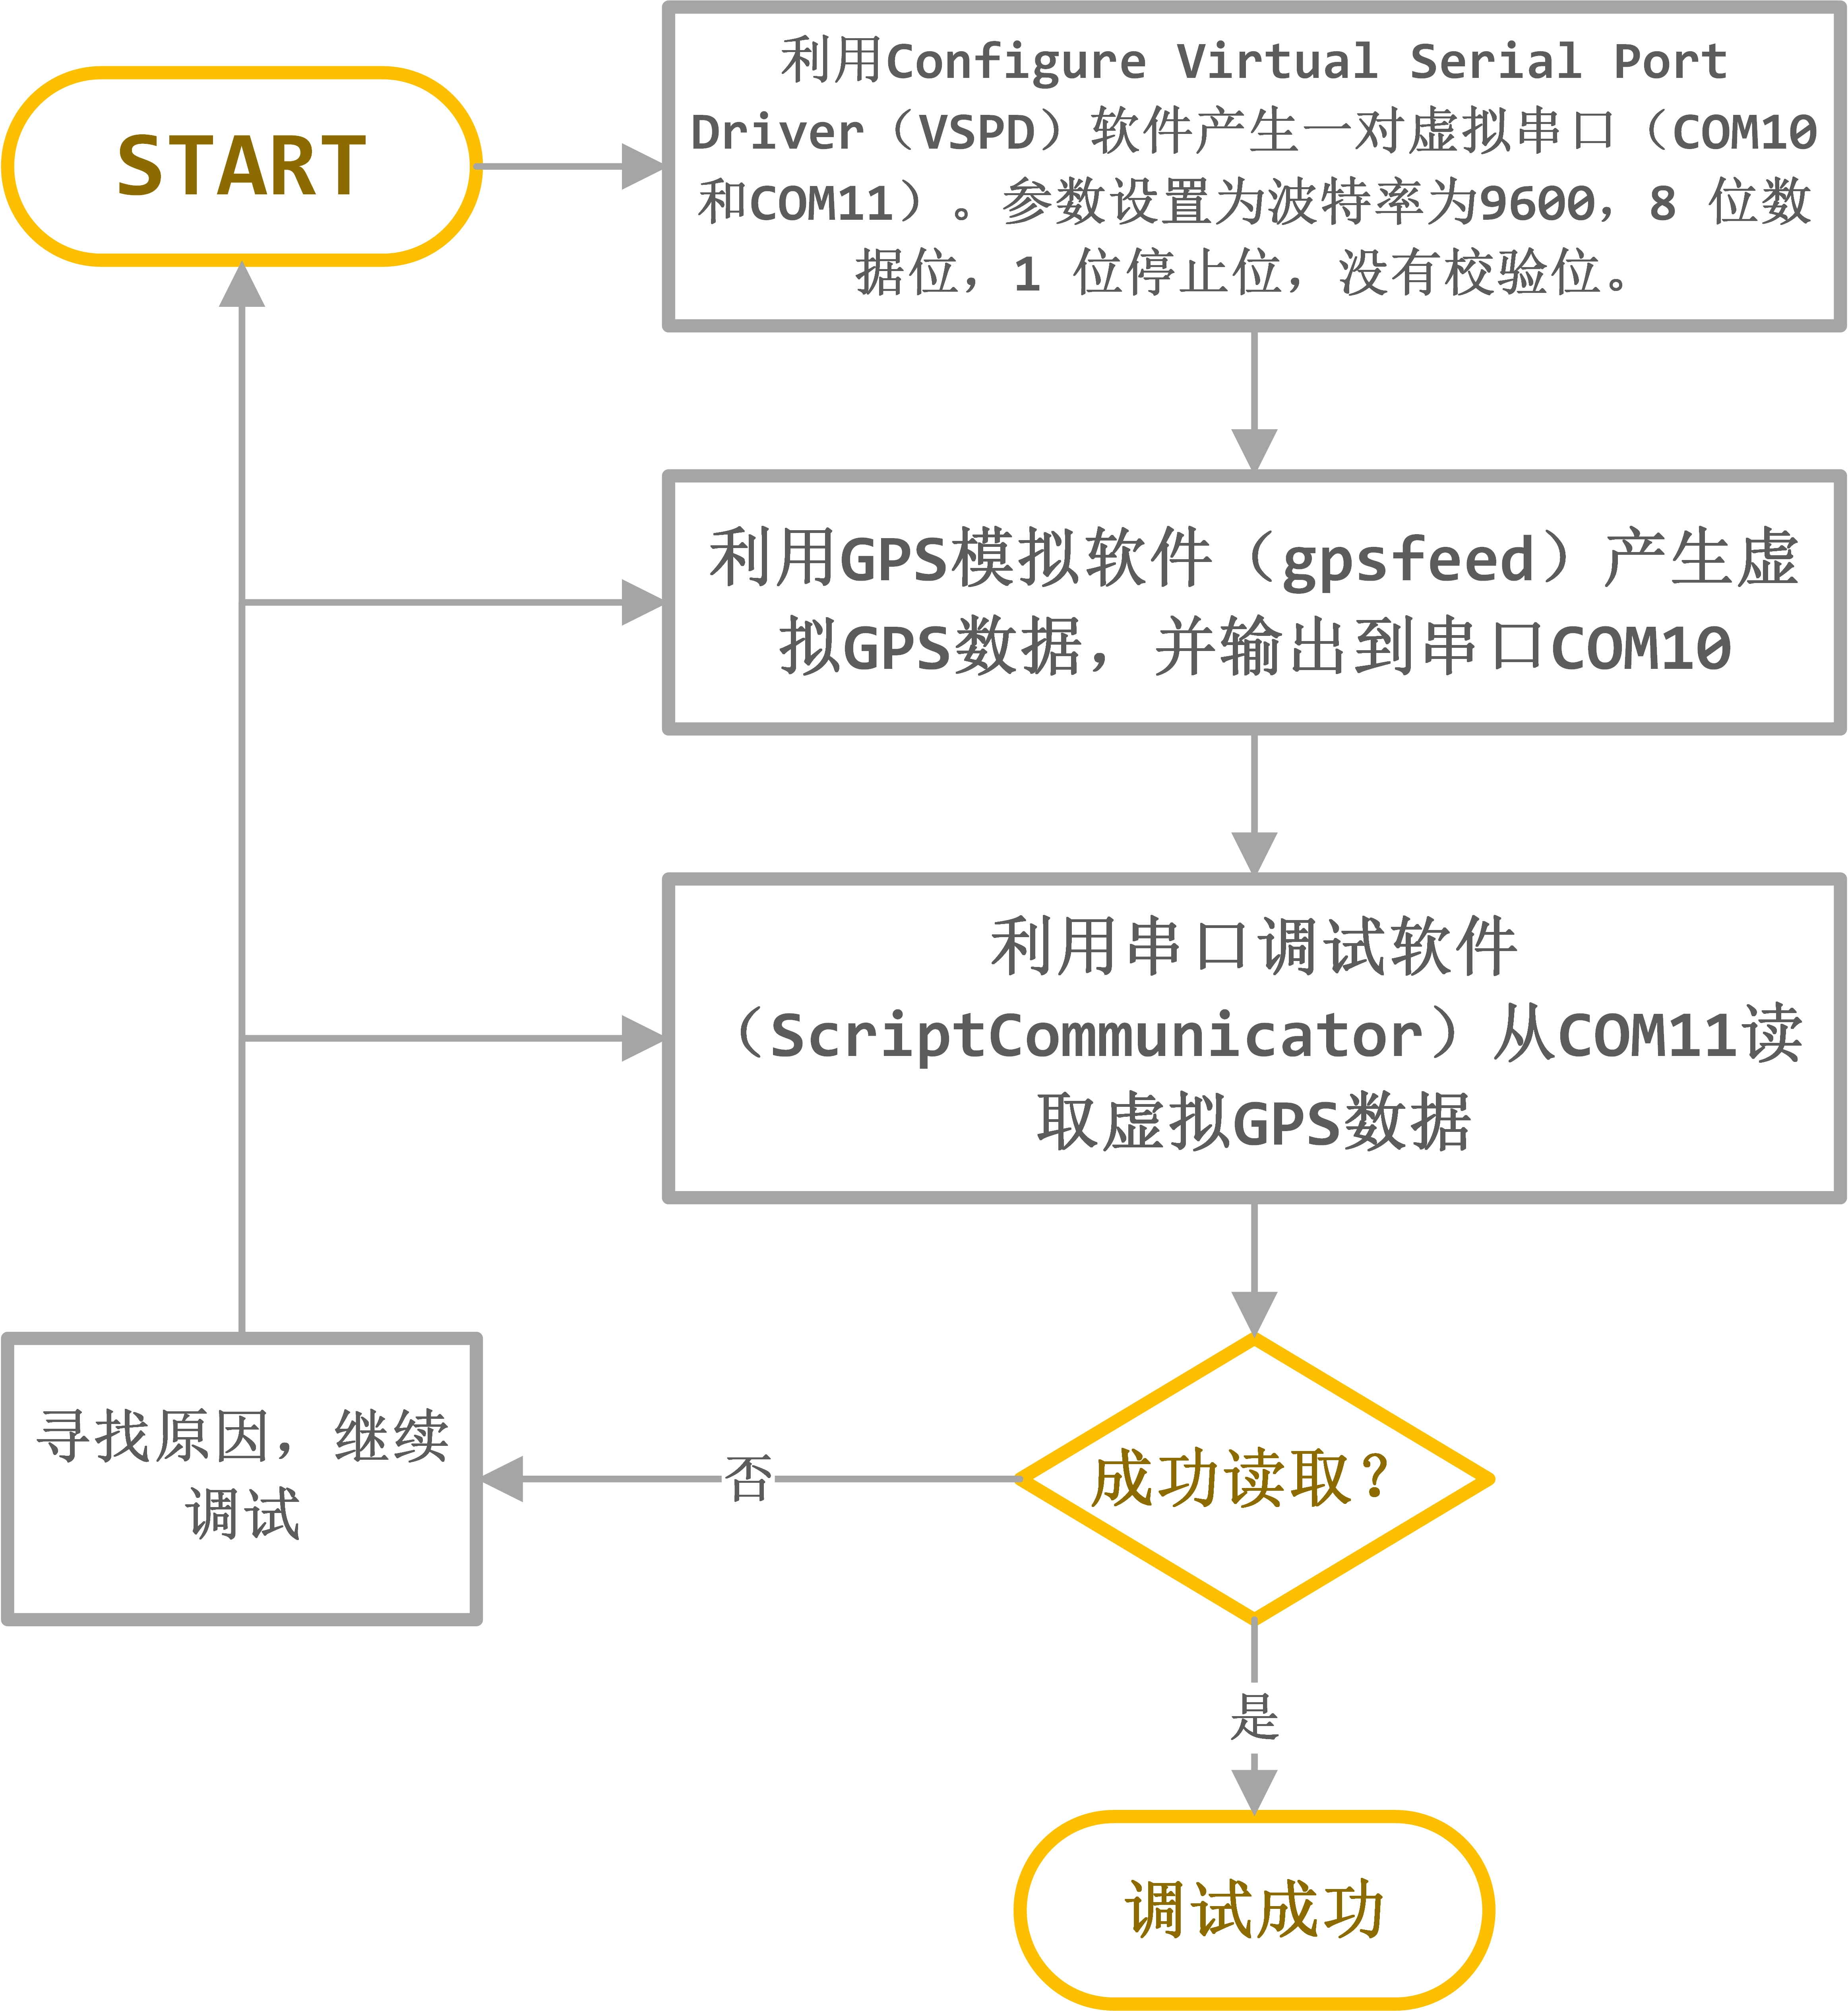
\includegraphics[width=10cm]{figs/f1.jpg}
    \caption{搭建虚拟环境流程图}
    \label{f1}
\end{figure}
\subsection{产生虚拟串口}

下载安装Configure Virtual Serial Port Driver(VSPD)软件,
VSPD界面如图(\ref{f2})所示。
\begin{figure}[htbp]
    \centering
    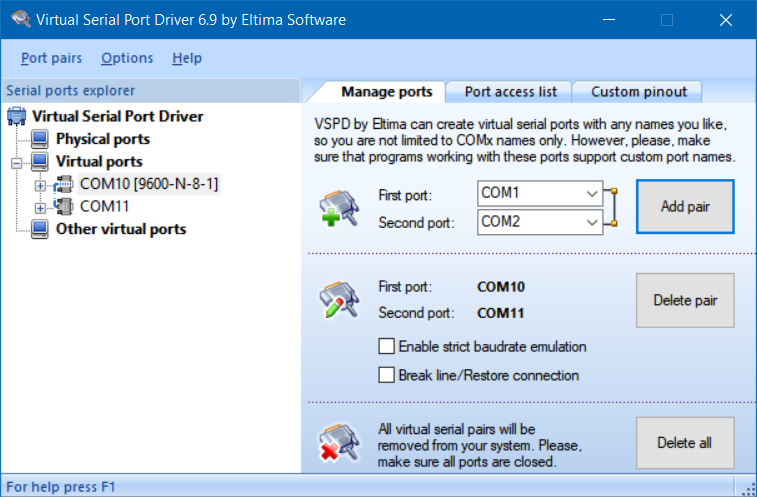
\includegraphics[width=10cm]{figs/f2.png}
    \caption{VSPD界面}
    \label{f2}
\end{figure}
在此处产生一对端口,分别为COM10和COM11。

并检查是否配置成功,打开电脑的设备管理器,如下图(\ref{f3})所示。
可以看到COM10和COM11被成功配置。
\begin{figure}[htbp]
    \centering
    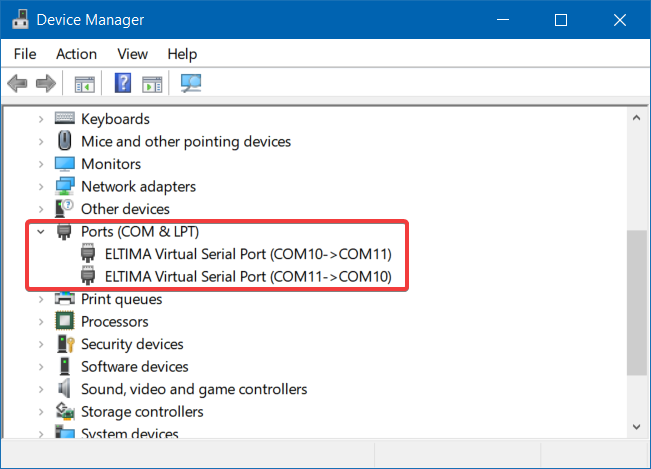
\includegraphics[width=10cm]{figs/f3.png}
    \caption{COM10和COM11被成功配置}
    \label{f3}
\end{figure}
\subsection{产生虚拟GPS数据}
下载GPS模拟器gpsfeed+,并配置好参数,如下图(\ref{f45})所示。
\begin{figure}[htbp]
    \centering
    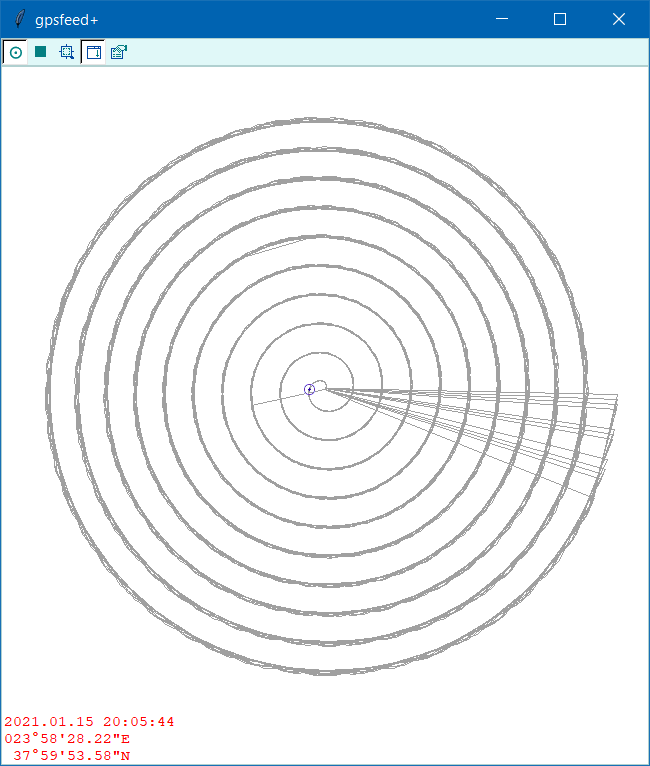
\includegraphics[height=7cm]{figs/f4.png}
    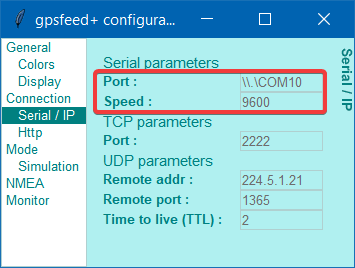
\includegraphics[height=7cm]{figs/f5.png}
    \caption{gpsfeed+界面图和参数配置}
    \label{f45}
\end{figure}

配置gpsfeed+将其产生的虚拟GPS数据发送到COM10串口,并配置波特率为9600。

在填写串口时,应写为\verb|\|\verb|\|.\verb|\|COM??。因为
gpsfeed+是用TCL语言开发的,
它打开串口用的是puts命令,
而puts命令是通过Windows API
的CreateFile函数实现的。CreateFile函数只能打开COM1$\sim$COM9,
而对于大于9的COM口,需要采用“\verb|\|\verb|\|.\verb|\|COM??”的格式打开$\text{}^{[2]}$。

\subsection{调试串口}
下载串口调试工具ScriptCommunicator,配置其接收串口为COM11,波特率
为9600,可以正常接收到数据,如下图(\ref{f6})所示。
\begin{figure}[htbp]
    \centering
    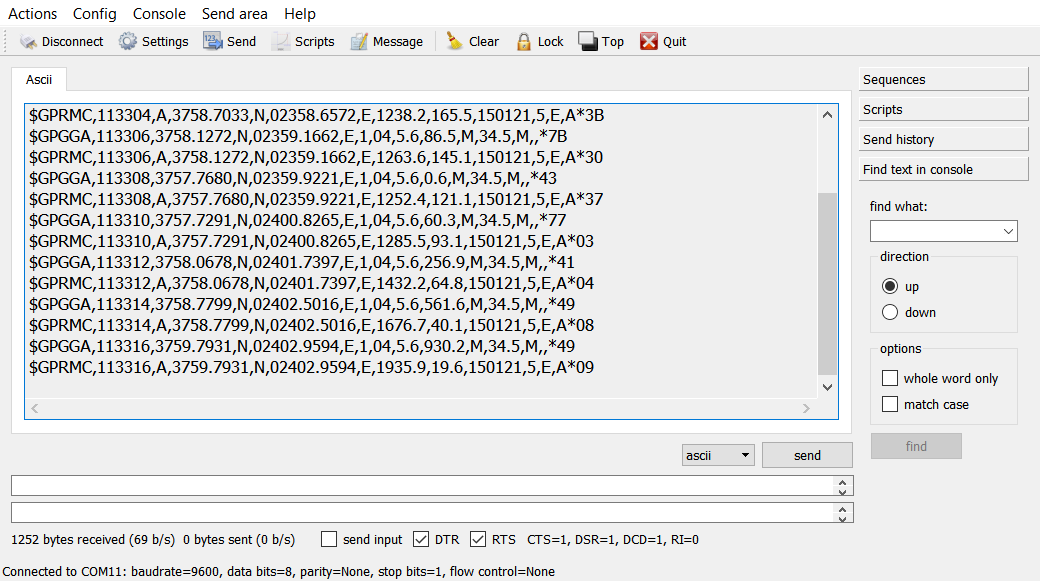
\includegraphics[width=10cm]{figs/f6.png}
    \caption{ScriptCommunicator从串口COM11读取数据}
    \label{f6}
\end{figure}
\section{程序设计}

\subsection{程序设计框图}
程序设计框图如下图(\ref{f7})所示。
\begin{figure}[htbp]
    \centering
    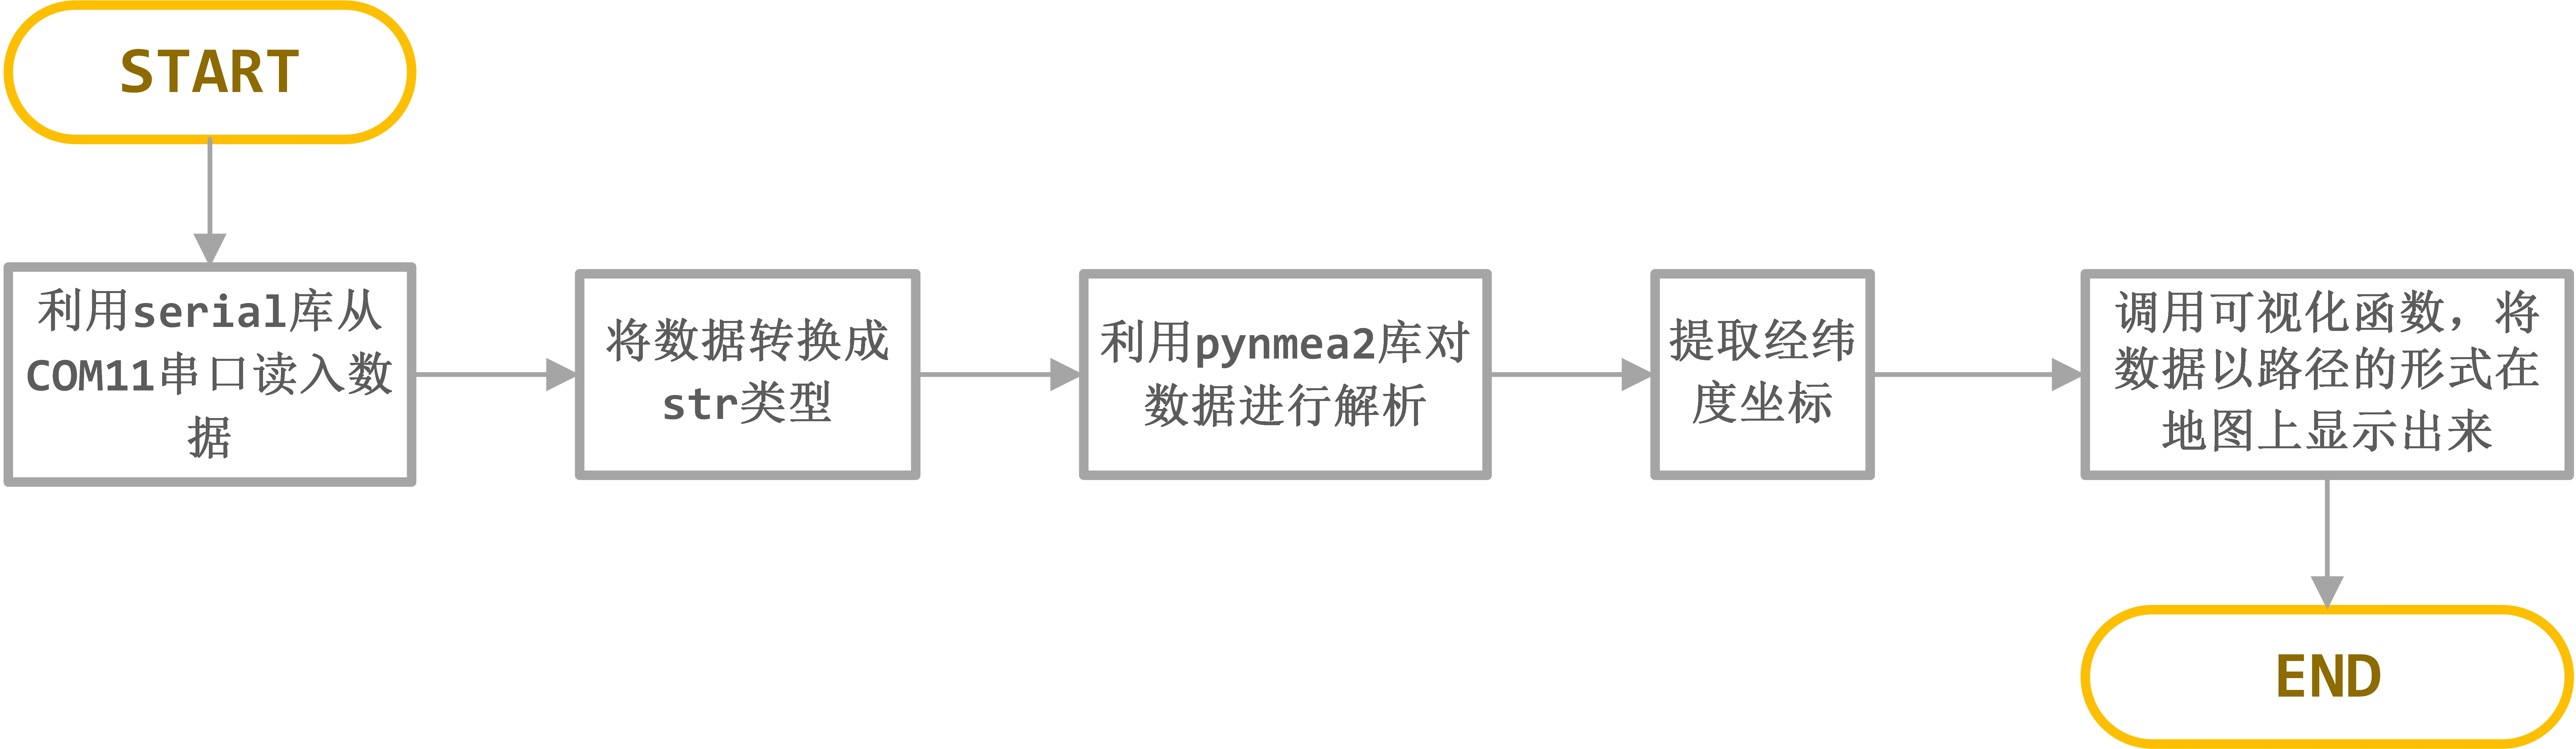
\includegraphics[width=15cm]{figs/f7.jpg}
    \caption{Python程序设计框图}
    \label{f7}
\end{figure}

在此程序中,主要利用了两个Python库,分别为serial和pynmea2库。
通过serial库可以从串口读取数据;通过pynmea2库可以对GPS数据进行解析,
进而得到经纬度坐标。
\subsection{程序设计过程}
1. 利用serial库打开串口
\begin{lstlisting}[
	language = python, numbers=left, 
	numberstyle=\tiny,keywordstyle=\color{blue!70},
	commentstyle=\color{red!50!green!50!blue!50},frame=shadowbox,
	rulesepcolor=\color{red!20!green!20!blue!20},
	basicstyle=\ttfamily,
	]
ser = serial.Serial(
    port='COM11',
    baudrate=9600, 
    bytesize=8, 
    parity='N', 
    stopbits=1) 
\end{lstlisting}

2. 读取数据并将数据转换为str类型
\begin{lstlisting}[
	language = python, numbers=left, 
	numberstyle=\tiny,keywordstyle=\color{blue!70},
	commentstyle=\color{red!50!green!50!blue!50},frame=shadowbox,
	rulesepcolor=\color{red!20!green!20!blue!20},
	basicstyle=\ttfamily,
	]
data=ser.readline()
data_str=str(data,encoding="utf-8")
\end{lstlisting}

3. 利用pynmea2库对数据进行解析
\begin{lstlisting}[
	language = Python, numbers=left, 
	numberstyle=\tiny,keywordstyle=\color{blue!70},
	commentstyle=\color{red!50!green!50!blue!50},frame=shadowbox,
	rulesepcolor=\color{red!20!green!20!blue!20},
	basicstyle=\ttfamily,
	]
msg=pynmea2.parse(data_str)
\end{lstlisting}

4. 提取经纬度坐标
\begin{lstlisting}[
	language = Python, numbers=left, 
	numberstyle=\tiny,keywordstyle=\color{blue!70},
	commentstyle=\color{red!50!green!50!blue!50},frame=shadowbox,
	rulesepcolor=\color{red!20!green!20!blue!20},
	basicstyle=\ttfamily,
    ]
location0=[msg.latitude,msg.longitude]
location.append(location0)
\end{lstlisting}

5. 将数据显示在地图上
\begin{lstlisting}[
	language = Python, numbers=left, 
	numberstyle=\tiny,keywordstyle=\color{blue!70},
	commentstyle=\color{red!50!green!50!blue!50},frame=shadowbox,
	rulesepcolor=\color{red!20!green!20!blue!20},
	basicstyle=\ttfamily,
    ]
draw_gps(location, path,'f3.html')
\end{lstlisting}

\newpage
\section{结果分析}

\begin{enumerate}
    \item 设置程序从串口读入10个GPS数据,得到纬度和经度坐标,
    并将此数据显示在地图上,得到的路径如下图所示(\ref{f8}),在希腊雅典附近。
\begin{figure}[htbp]
    \centering
    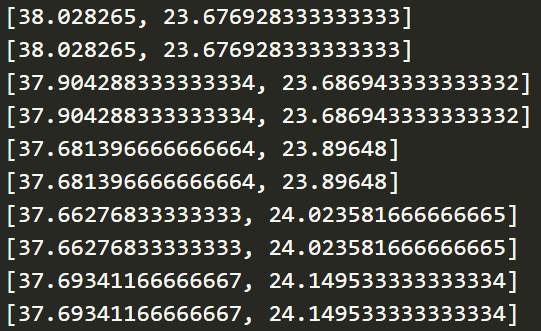
\includegraphics[height=5.3cm]{figs/f8.png}    
    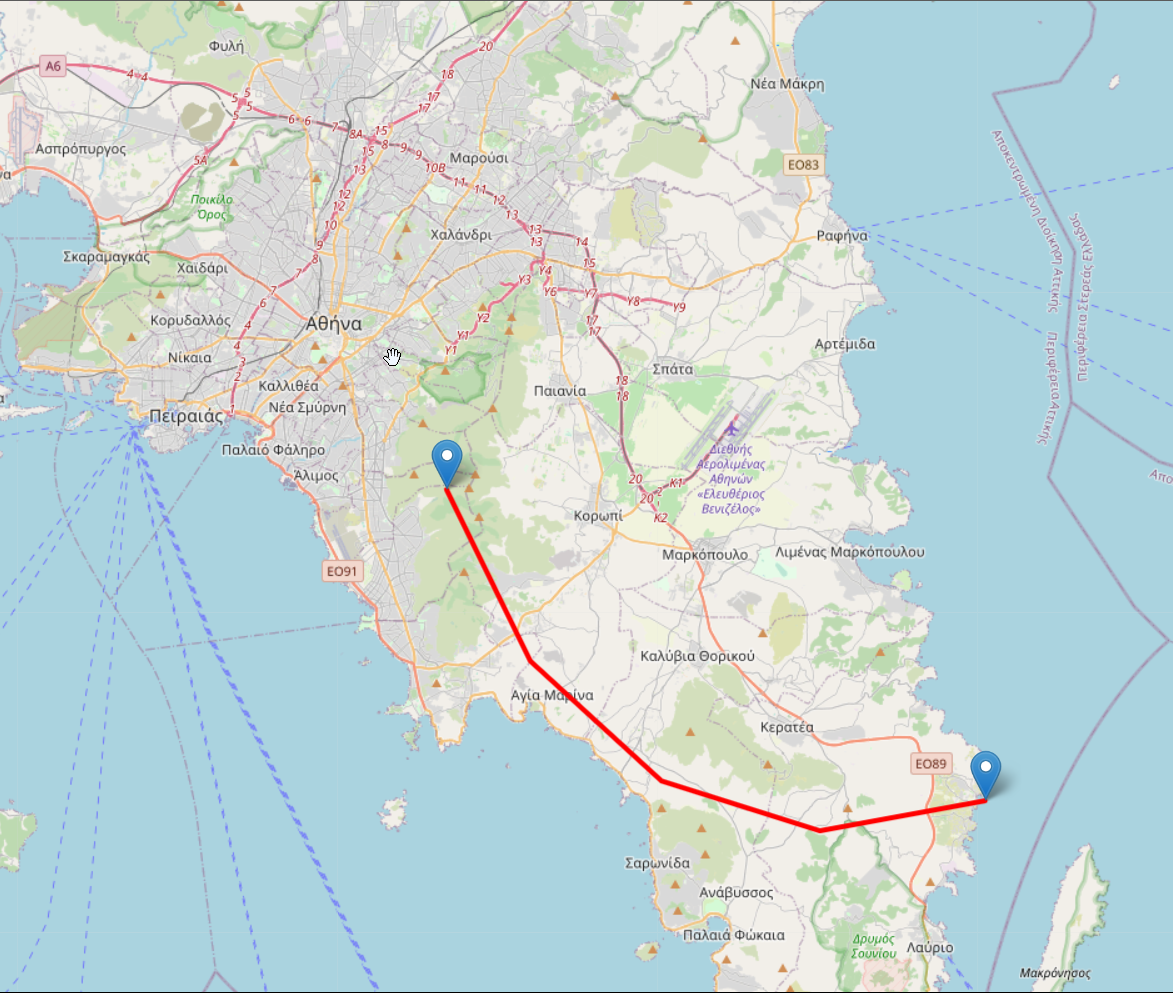
\includegraphics[height=5.3cm]{figs/f14.png}
    \caption{从串口读取的10个纬度经度坐标及路径}
    \label{f8}
\end{figure}



\item 设置程序从串口读入100个GPS数据,得到纬度和经度坐标,
并将此数据显示在地图上,得到的路径如下图(\ref{f10})所示。
\begin{figure}[htbp]
    \centering
    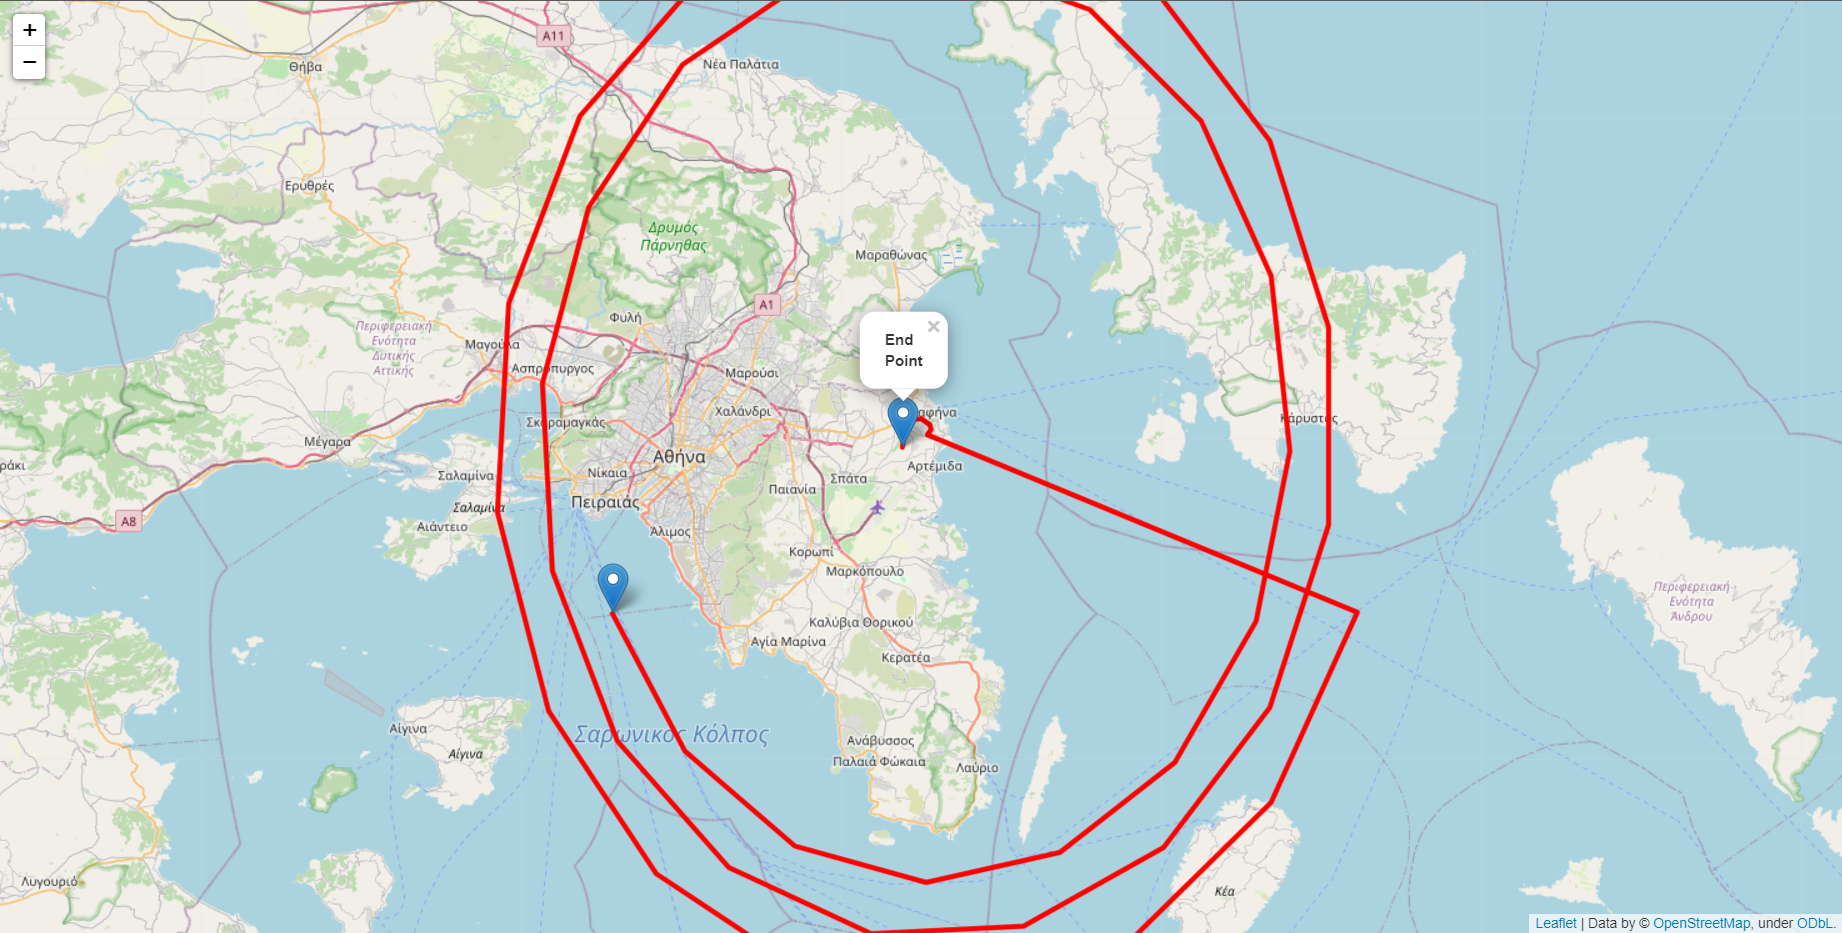
\includegraphics[width=15cm]{figs/f9.png}
    \caption{从串口读取的100个纬度经度所绘制的路径}
    \label{f10}
\end{figure}

\item 设置程序从串口读入1000个GPS数据,得到纬度和经度坐标,
并将此数据显示在地图上,得到的路径如下图(\ref{f11})所示。
\begin{figure}[htbp]
    \centering
    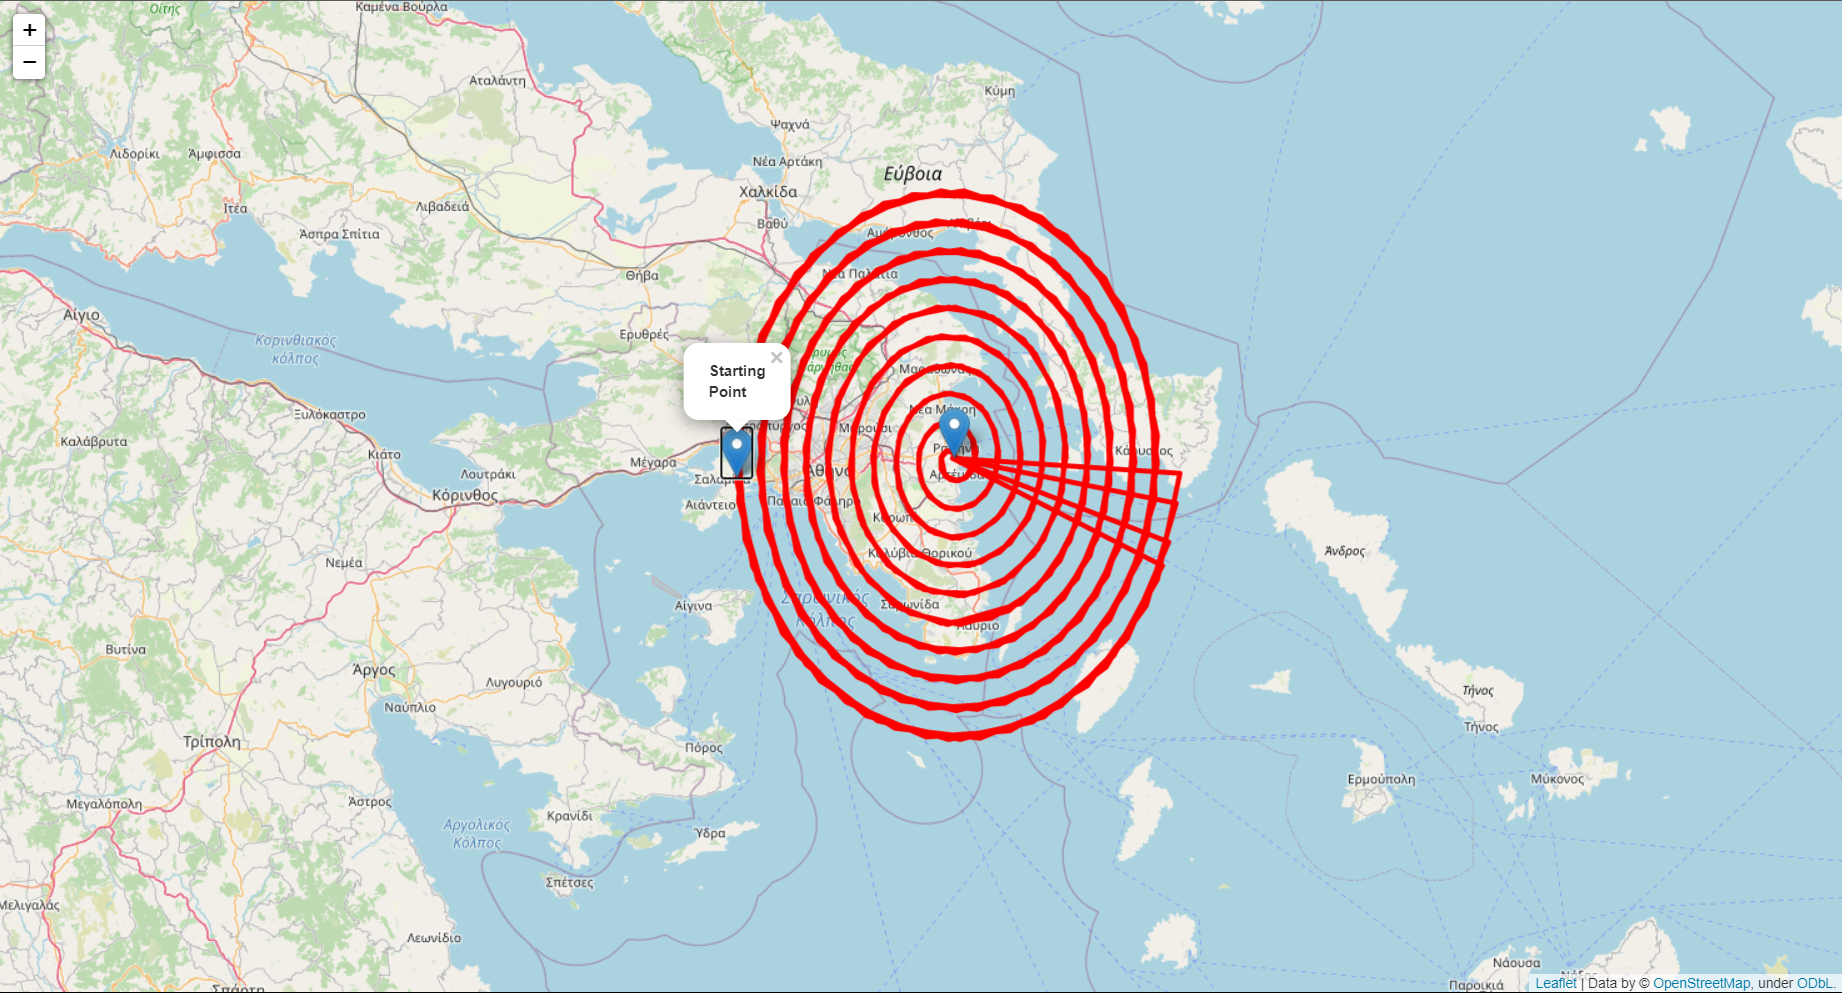
\includegraphics[width=15cm]{figs/f13.png}
    \caption{从串口读取的1000个纬度经度所绘制的路径}
    \label{f11}
\end{figure}
\end{enumerate}




\section{结论}

本文利用了Python实现了NMEA-0183协议下GPS数据的串口通讯程序设计,
并对数据进行了可视化显示,将路径显示在了地图上。

同时搭建了虚拟串口并利用GPS模拟器产生了虚拟的GPS数据,
便于对本程序进行验证和测试。

在编写程序的过程中,遇到了一些困难,在此一一列出并说明如何解决。
\begin{enumerate}
    \item 在产生虚拟串口时,运用老师推荐的com0com虚拟串口软件时,虽然设备管理器已经检测到了串口,
    但因为一些不可知的原因,
    设备管理器中显示串口不可用。
    无奈之下重新下载了虚拟串口软件Configure Virtual Serial Port Driver(VSPD),使此问题得到解决
    \item 在gpsfeed+产生虚拟GPS数据时,发现软件并没有将数据输出到串口,而是输出到了本地文件,
    其他同学也遇到了此问题,但通过按照李老师所撰写的推送(\href{https://mp.weixin.qq.com/s/sCODhan6wwRr1mklzY9Uqw}{gpsfeed+如何使用编号大于9的串口})
    中的步骤操作,解决了此问题。
    \item 在进行Python程序编写的过程中,发现接收到的串口数据并不是str的数据类型,而是bytes类型,不能
    直接通过pynmea2库进行处理,因此利用$str()$语句将bytes型转换为str型,问题得到解决。
\end{enumerate}

在完成此项目的过程中,更加意识到了Python语言的强大,利用C语言需要几十行的代码,但利用Python
可能只需要几行即可解决,因此以后要在数据分析,深度学习等重要领域加强对Python语言的掌握。

\section{参考文献}

\noindent [1] 韩友美,钟政,桑逢云. NEMA—0183协议下GPS数据的实时串口通讯程序设计[A]. 山东土地学会、山东测绘学会.山东省“数字国土”学术交流会论文集[C].山东土地学会、山东测绘学会:山东省科学技术协会,2007:4.

\noindent [2] \href{https://mp.weixin.qq.com/s/sCODhan6wwRr1mklzY9Uqw}{gpsfeed+如何使用编号大于9的串口}

\end{document}